\chapter{ Практическое применение предлагаемой методики тестирования } \label{ch4}

В данной главе описывается порядок апробации предложенной методики сравннительного тестирования реализаций алгоритмлв путем сравнительного тестирования пропускной способности трех реализаций алгоритма AES на языке С. Анализируются результаты тестирования.
	
\section{Инфраструктура тестирования и обработки результатов} \label{ch4:sec1}

Реализация избранного алгоритма AES исполнена на языке Си. Выбран не ассемблер, так как Си значительно проще для реализации и отладки, а трансляцию его команд в ассемблер несложно увидеть, например, с использованием средств отладки IDE Visual Studio. Данный алгоритм выбран по причине его высокой стойкости, сочетающейся с существованием достаточно легковесных реализаций. Впрочем, предложенным способом может быть протестирован любой криптоалгоритм.

Также используются некоторые библиотеки языков C и C++. Это модуль time.h для измерения времени, модуль windows.h для точного измерения времени, а также stdlib.h для получения псевдослучайных чисел и vector.h для удобной работы с массивами переменной длины.

Тестированию подвергаются три реализации алгоритма AES на языке Си. Это две реализации, взятые из открытых источников (~\cite{src72,src73}), а также авторская реализация. Все три реализации были предварительно протестированы. Разработка авторской версии велась с упором на компактность кода и минимизацию «лишних» операций и потребления ОЗУ. На её основе может быть создана ассемблерная реализация. Причем тестировать ее можно с использованием того же окружения С/С++. В этом случае необходимо использовать массив чисел – опкодов процессорных команд.

Порядок тестирования времени исполнения таков. Для каждого алгоритма производится n серий измерений времени шифрования. На каждой из серий производится m измерений для различных объемов $V_i$ входных данных, $i=1…m$. Под входными данными понимается набор случайно сгенерированных блоков (количеством $V_i$), которые последовательно подвергаются шифрованию, ключ для каждого блока свой, он тоже генерируется случайно. Для уменьшения влияния погрешности, каждое измерение выполняется t раз, время суммируется. Итого для каждого алгоритма имеется $n$ рядов по $m$ точек.

Необходимо принимать меры, предотвращающие «заоптимизирование» вызовов тестируемых функций, работающих «вхолостую». То есть требуется сделать так, чтобы оптимизатор не удалил блоки кода (вызов функции), результат которых никак не используется. Меры следующие:
\begin{enumerate}
	\item Есть специальный контрольный байт, значение которого обновляется при каждом шифровании (увеличивается на значение первого байта шифротекста). Он выводится в консоль. Время обновления контрольного байта и вывода его на экран в общем времени не учитывалось.
	\item На каждом из $t$ измерений используются разные входные данные (но одного объема).
\end{enumerate} 

Еще одна особенность тестирования в том, что при большом количестве вызовов одной и той же функции подряд время ее исполнения уменьшается. Возможно, это связано с тем, что Windows требуется время, чтобы предоставить все требуемые ресурсы. Этот эффект оказывает влияние на результаты тестирования, причем чем больше объем данных, тем это влияние сильнее. Учесть его влияние не представляется возможным. К счастью, в данном тестировании его влияние не так велико, как могло бы быть, поскольку тестируемые алгоритмы планируется использовать для шифрования пакетов данных небольшого размера. 

Следующим этапом идет обработка результатов измерения. Она производится на языке Python. Затем для каждой из серий измерений по $m$ точкам строится прямая $y=kx+b$. Она строится с помощью метода наименьших квадратов. Фиксируются ее значения $k$ и $b$ и их погрешности. Таким образом фиксируются $n$ пар $k$ и $b$. Наконец, вычисляется итоговые значения $k$ и $b$. Это и будут пропускная способность и задержка алгоритма, соответственно.

\section{Результаты тестирования} \label{ch4:sec2}

При тестировании использовались следующие параметры.

\begin{center}
	\begin{tabular}{ | c | c | }
		\hline
		Параметр & Значение \\ \hline
		$n$ & 10 \\ \hline
		$t$ & 100 \\ \hline
		$m$ & 11 \\ \hline
		$V_i$ & 10, 12, 14, 16, 18, 20, 22, 24, 26, 28, 30 \\
		\hline
	\end{tabular}
\end{center}

Для алгоритма AES размер блока составляет 128 бит (16 байт), размер ключа также 128 бит.

Полученные данные (временной ряд 1) для каждой из трех реализаций приводится на рис. 4.1-4.3. Можно видеть, что точки весьма хорошо ложатся на прямую, как и следовало ожидать. В реализациях 1 и 2 первый тест первой серии занимает больше времени, чем следует из теоретической модели. Возможно, это связано с тем, что Windows требуется время, чтобы предоставить все требуемые ресурсы.

\begin{figure}[ht!] 
	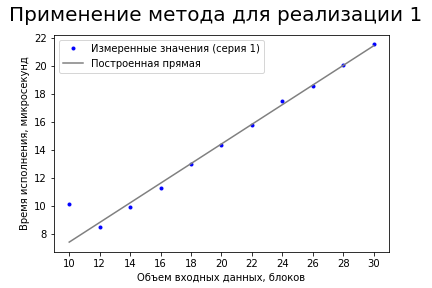
\includegraphics [scale=0.8] {my_folder/plots//plot1}
	\centering
	\caption{Применение метода для реализации 1} 
\end{figure}

\begin{figure}[ht!] 
	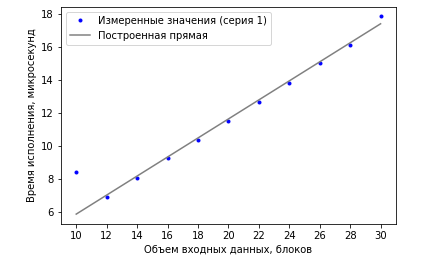
\includegraphics [scale=0.7] {my_folder/plots//plot2}
	\centering
	\caption{Применение метода для реализации 2} 
\end{figure}

\begin{figure}[ht!] 
	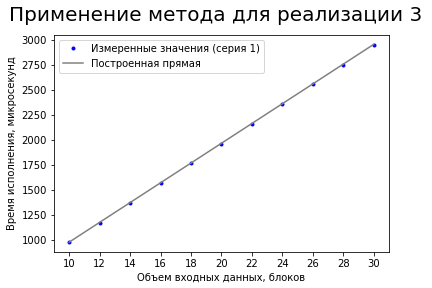
\includegraphics [scale=0.7] {my_folder/plots//plot3}
	\centering
	\caption{Применение метода для реализации 3} 
\end{figure}

Для сравнения, на рис. 4.4 приводятся данные для реализации 1 с увеличенным числом блоков (примерно на порядок). Против ожидания, результаты не исказились: точки по-прежнему соответствуют теоретической модели, причем восстановленные коэффициенты прямой получены почти такие же (см. далее). Это говорит в пользу предложенной методологии: она устойчива к увеличению объема входных данных. Исследовано поведение до объема 600 блоков (9.6 Кб). Дальнейшее увеличение представляется нецелесообразным, так как низкоресурсные устройства обычно не передают пакетов такого большого размера.

\begin{figure}[ht!] 
	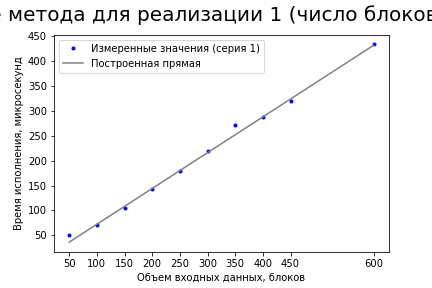
\includegraphics [scale=0.7] {my_folder/plots//plot4}
	\centering
	\caption{Применение метода для реализации 1 (число блоков увеличено)} 
\end{figure}

Также на рис. 4.1-4.4 приводятся усредненные экстраполированные прямые. Они демонстрируют неплохую робастность (устойчивость к выбросам, регулярно появляющимся при тестировании алгоритмов). Так, на рис. 4.4 точка, соответствующая 350 блокам, является выбросом.

Восстановленные уравнения прямых (для объемов 10-30 блоков):

\begin{equation}
y1 = 0.7x + 0.39
\end{equation}
\begin{equation}
y2 = 0.58x + 0.14
\end{equation}
\begin{equation}
y3 = 98.5x - 3.
\end{equation}

Восстановленные уравнения прямых (для объемов 50-600 блоков):

\begin{equation}
y1 = 0.72x + 0.68
\end{equation}
\begin{equation}
y2 = 0.61x - 1.3
\end{equation}
\begin{equation}
y3 = 100.3x - 37.9
\end{equation}

Как указано выше, коэффициент при х – пропускная способность алгоритма (микросекунд на блок), свободный член – время инициализации (микросекунд). Как видно, полученные значения пропускной способности достаточно стабильны на всех протестированных значениях. Время инициализации в действительности нулевое (поскольку алгоритм не потоковый, а блочный), поэтому оно значительно колеблется как по модулю, так и по знаку. Также, возможно, на него оказывает влияние планировщик Windows: с течением времени выделяет все больше и больше ресурсов на данную задачу.

Значения пропускной способности для реализаций 1 и 2 достаточно близки (0.7 и 0.6 микросекунд на блок соответственно). Они равны 23 Мб/с и 26 Мб/с, соответственно. Пропускная способность реализации 3 значительно меньше (100 микросекунд на блок, т. е. 0.16 Мб/с).

В качестве причин столь низкой производительности можно выделить отказ от чтения табличных данных (которые занимают оперативную память) и вместо этого вычисление этих данных. Второй причиной является «in-place» параметр, т.е. результат шифрования записывается по тому же указателю, из которого читаются входные данные. Это делает невозможной раскрутку циклов (которую выполняет оптимизатор), то есть очередная итерация не может начаться раньше, чем закончится предыдущая. Для тестирования алгоритмов, нацеленных на легковесную реализацию, такой режим тестирования гораздо более предпочтителен, так как уменьшает влияние процессорных оптимизаций, в том числе внутреннего параллелизма.

\section{Выводы} \label{ch4:conclusion}

В данной главе был описан порядок апробации предложенной методики сравннительного тестирования реализаций алгоритмлв путем сравнительного тестирования пропускной способности трех реализаций алгоритма AES на языке С. Проанализированы результаты тестирования.

\newpage

%% Вспомогательные команды - Additional commands
%
%\newpage % принудительное начало с новой страницы, использовать только в конце раздела
%\clearpage % осуществляется пакетом <<placeins>> в пределах секций
%\newpage\leavevmode\thispagestyle{empty}\newpage % 100 % начало новой страницы